\documentclass[handout]{beamer}

\usepackage[italian]{babel}
\usepackage{minted}
\usepackage{mdframed}

\surroundwithmdframed{minted}

\newminted{cpp}{linenos,autogobble,breaklines}

\newcommand{\scaledimage}[1]{\includegraphics[width=\textwidth,height=0.8\textheight,keepaspectratio]{#1}}

\usetheme{Boadilla}
\title{02 - Recap}
\author{Bailetti Tommaso}
\institute{ITI Don Orione}
\date{3 Febbraio 2022}

\begin{document}
    \begin{frame}
        \titlepage
    \end{frame}

    \begin{frame}
        \frametitle{Le variabili}
        Le variabili sono il nostro modo di inserire all'interno del nostro programma dei "valori". Al momento dell'esecuzione vengono allocati in memoria i \texttt{byte} necessari per tutte le nostre variabili.
    \end{frame}
    
    \begin{frame}
        \frametitle{Tipo di variabili}
        Il programmatore necessita di sapere cos'è il \textbf{tipo} di una variabile. Il tipo non è che la definizione di \textbf{cosa} stiamo salvando all'interno della variabile. Ci sono differenti tipi di variabili in C++.
    \end{frame}
    
    \begin{frame}
        \frametitle{Tipo di variabili}
        \begin{center}
            \scaledimage{img/types.png}
        \end{center}
    \end{frame}

    \begin{frame}
        \frametitle{Ulteriori keyword per le variabili}
        Per le variabili sono presenti due ulteriori keyword che permettono di modificare le definizioni delle nostre variabili:
        \begin{description}
            \item[\texttt{signed/unsigned}]<2-> Ci permette di definire se la nostra variabile deve mantenere il segno o meno.
            \item[\texttt{const}]<3-> Ci permette di definire e inizializzare una variabile il quale valore non è mai modificato durante l'esecuzione. 
        \end{description}
    \end{frame}

    \begin{frame}[fragile]
        \frametitle{Quindi in sostanza, per dichiarare una variabile}
        \begin{center}
            \Large{\texttt{*const* *unsigned* <tipo> <nomeVariabile>;}}
        \end{center}
        dove le keyword tra gli asterischi sono opzionali, a seguire degli esempi
        \begin{center}
            \begin{cppcode}
                const float pi = 3.14;
                unsigned int numberOfResets = 0;
                char yesChar = 'Y';
            \end{cppcode}
        \end{center}
    \end{frame}

    \begin{frame}
        \frametitle{Scope and Lifetime}
        Ora che sappiamo cosa sono le variabili, è necessario approfondire cosa sono lo "scope" e il "lifetime" di una variabile.
    \end{frame}

    \begin{frame}
        \frametitle{Scope}
        L'\textbf{ambito di visibilità} o \texttt{scope} è il blocco di istruzioni dove la nostra variabile è dichiarata. Al di fuori di essa la nostra variabile di fatto non esiste più. Le variabili possono quindi essere:
        \begin{description}
            \item[Variabili Globali]<2-> È valida dall'inizio dell'esecuzione del software fino al termine. Una variabile è di fatto globale solo se è definita al di fuori di un blocco di istruzioni.
            \item[Variabili Locali]<3-> Sono valide solo all'interno del proprio blocco e non è possibile accedervi al di fuori di esso. 
        \end{description}
    \end{frame}

    \begin{frame}
        \frametitle{Lifetime}
        Il \textbf{tempo di vita} di una variabile o \texttt{lifetime} è il tempo per la quale la nostra variabile è presente all'interno del programma. Di fatto dipende da che \texttt{scope} diamo alla nostra variabile.
        \begin{description}
            \item[Variabile Permanente]<2-> \textit{una variabile globale è sempre permanente}, si crea all'inizio dell'esecuzione e rimane per tutta la durata dell'esecuzione.
            \item[Varaibile Temporanea]<3-> \textit{è allocata solamente all'inizio dell'esecuzione del blocco che ne comprende la dichiarazione}. Lo spazio in memoria, una volta eseguito il blocco, viene liberato dalla variabile.
        \end{description}
    \end{frame}

    \begin{frame}
        \frametitle{Matematica in C++}
        \begin{center}
            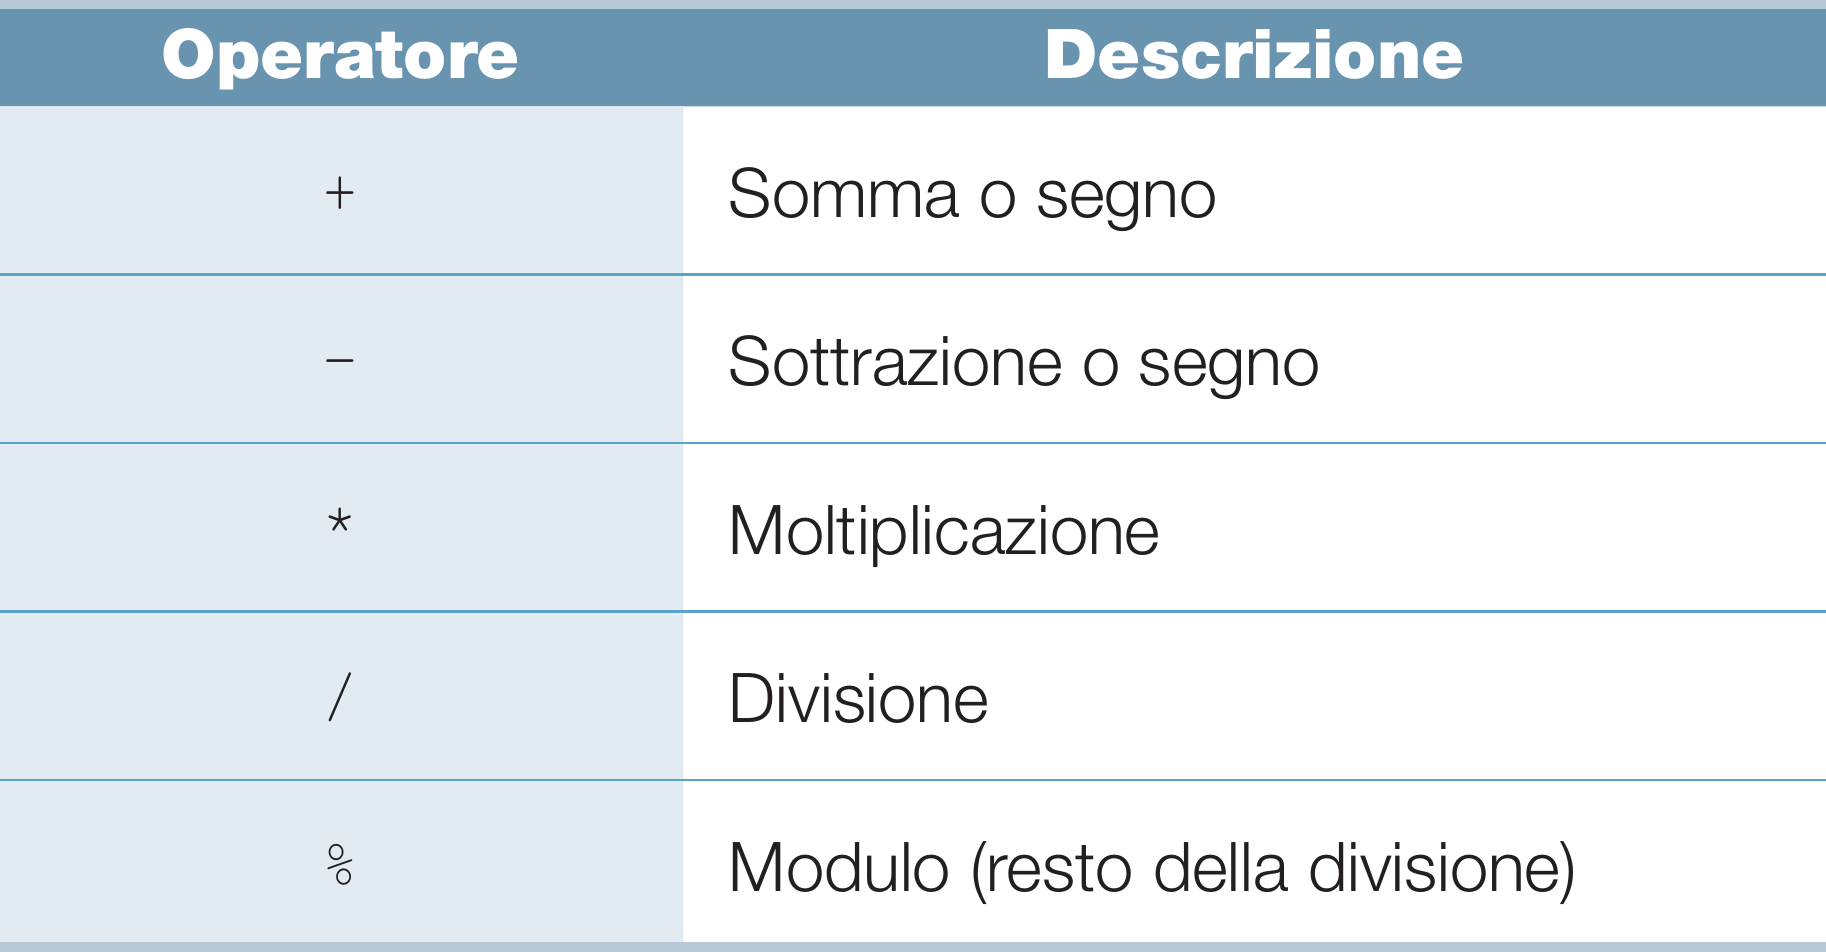
\includegraphics[scale=0.17]{img/operators.png}
        \end{center}
        \onslide<2->
        Un consiglio che vi dò, è quello di mettere sempre tra parentesi i calcoli nell'ordine in cui volete siano eseguiti. C++ usa le priorità "normali" della matematica (prima le moltiplicazioni e divisioni, poi le somme e sottrazioni) tuttavia prendiamo l'abitudine di non fidarci, può succedere che cambiando linguaggio di programmazione non sia più così.
    \end{frame}

    \begin{frame}[fragile]
        \frametitle{Operatori rapidi}
        Va menzionata anche la presenza di operatori matematici "compatti", i quali sono:
        \begin{table}
            \begin{tabular}{c | c}
                Versione Compatta & Versione Estesa \\
                \hline
                \mintinline{cpp}{a += b} & \mintinline{cpp}{a = a + b} \\
                \mintinline{cpp}{a -= b} & \mintinline{cpp}{a = a - b} \\
                \mintinline{cpp}{a *= b} & \mintinline{cpp}{a = a * b} \\
                \mintinline{cpp}{a /= b} & \mintinline{cpp}{a = a / b} \\
            \end{tabular}
        \end{table}
    \end{frame}

    \begin{frame}
        \frametitle{Incrementi}
        C++ mette a disposizione la possibilità di incrementare e decrementare le nostre variabili matematiche con la seguente sintassi:
        \begin{itemize}
            \item<2-> \texttt{<nomeVariabile>++} o \texttt{++<nomeVariabile>}
            \item<3-> \texttt{<nomeVariabile>--} o \texttt{--<nomeVariabile>}
        \end{itemize}
        \onslide<4-> di fatto questa cosa si traduce in:
        \begin{itemize}
            \item<4-> \texttt{<nomeVariabile> = <nomeVariabile> + 1} 
            \item<5-> \texttt{<nomeVariabile> = <nomeVariabile> - 1} 
        \end{itemize}
        
        \begin{block}<6->{Attenzione}
            con la sintassi \texttt{++<nomeVariabile>} e \texttt{--<nomeVariabile>} \textbf{l'operazione matematica avviene prima della interpretazione}.
        \end{block}
    \end{frame}

    \begin{frame}[fragile]
        \frametitle{Logica in C++}
        A questo punto dobbiamo imparare come far svolgere condizionalmente delle operazioni al nostro programma. Si possono effettuare comparazioni tra variabili e costanti con la seguente sintassi:
        \begin{center}
            \Large{\texttt{a <operatore> b}} \\
            \onslide<2-> 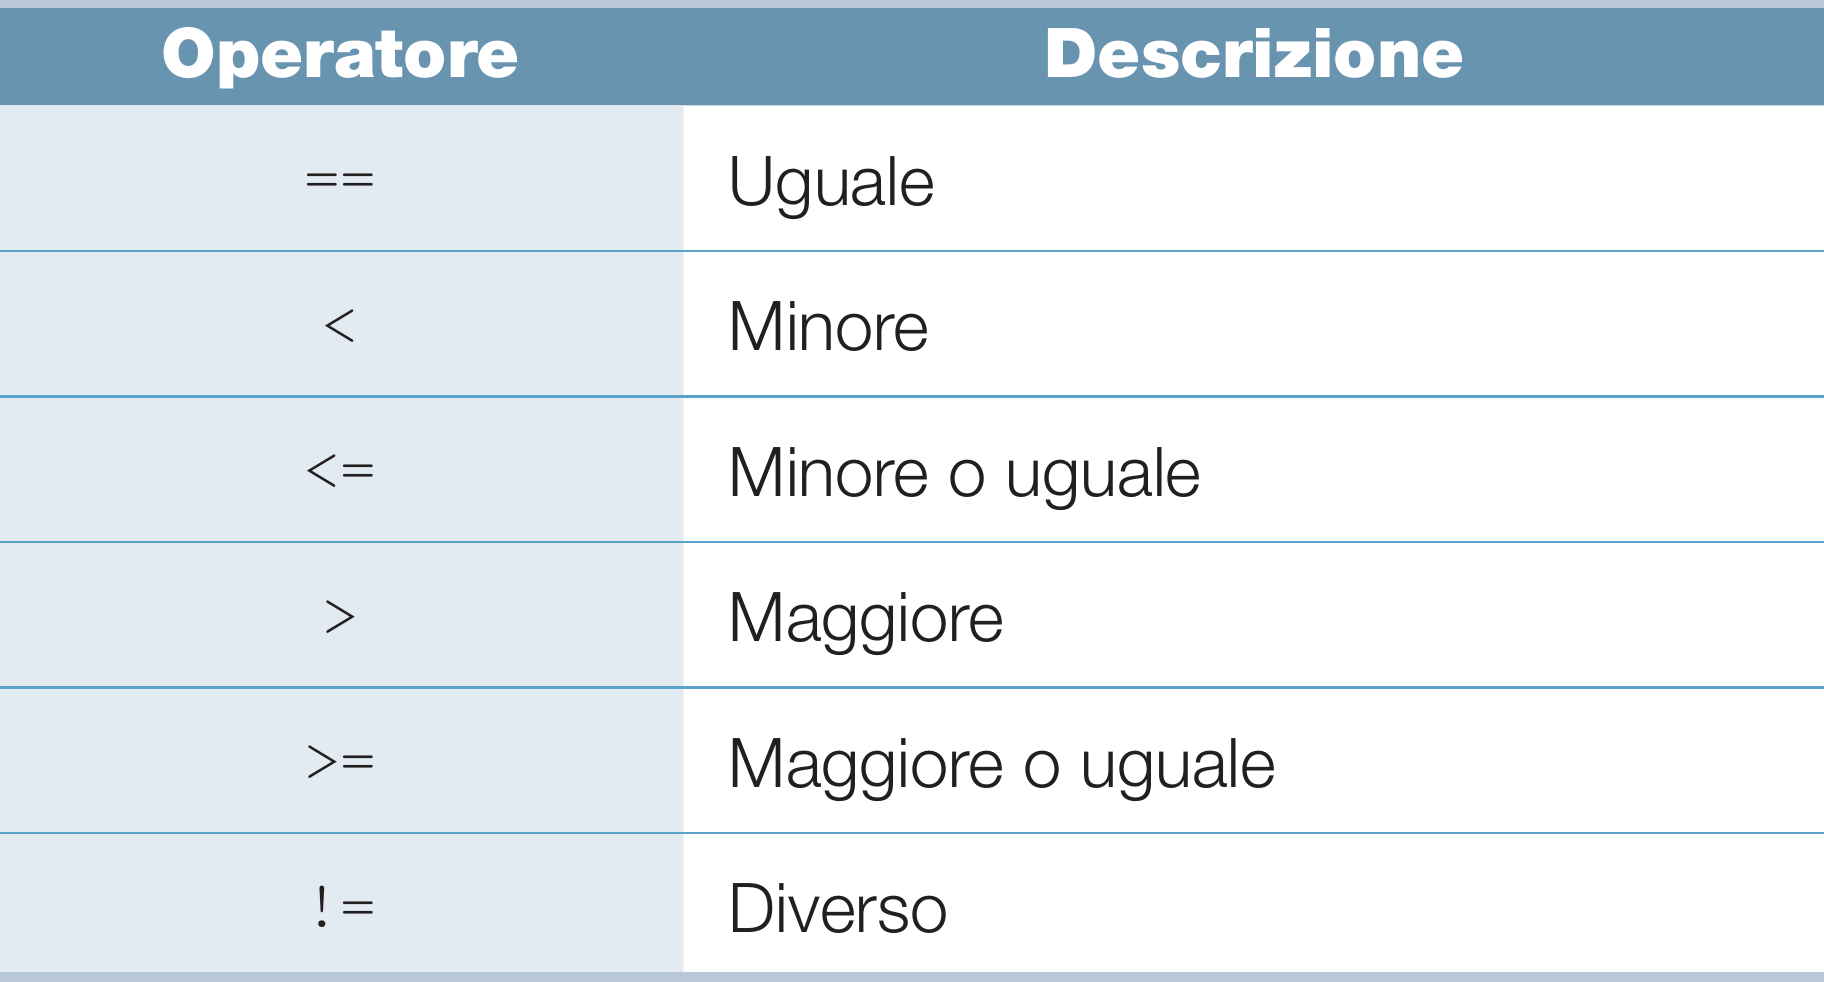
\includegraphics[scale=0.13]{img/logic_operators.png}
        \end{center}
        \begin{block}<3->{Nota bene}
            Tutte le comparazioni ritornano \mintinline{cpp}{true} o \mintinline{cpp}{false}.
        \end{block}
    \end{frame}

    \begin{frame}
        \frametitle{Espressioni Logiche}
        Inoltre le condizioni logiche possono essere combinate in un espressione logica, la quale pone il risultato della nostra condizione attraverso una porta logica.
        \begin{center}
            \onslide<2-> 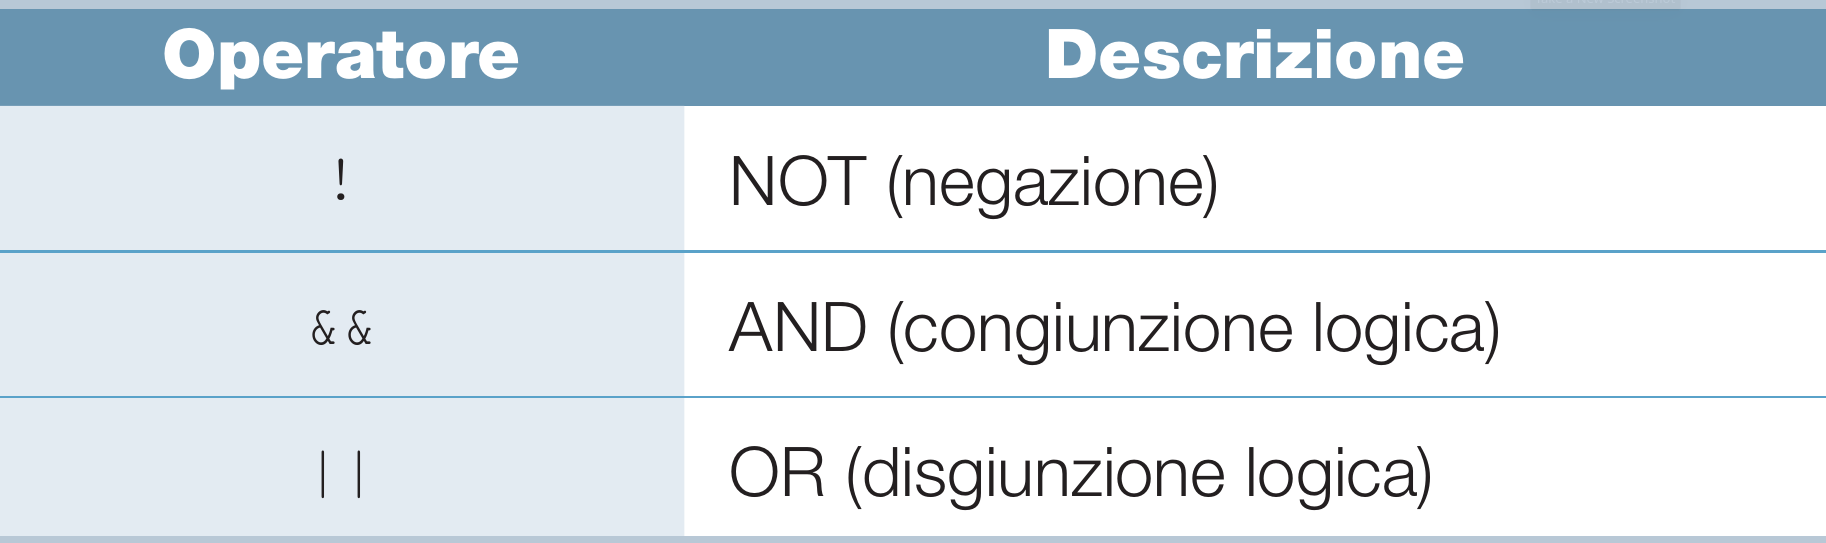
\includegraphics[scale=0.2]{img/logic_expressions.png}
        \end{center}
    \end{frame}

    \begin{frame}
        \frametitle{Casting}
        Il \texttt{cast} è una conversione fra tipi di variabili. Esistono due tipi di \texttt{casting} e sono condizionati dalla perdita o no dei dati durante il \texttt{cast}:
        \begin{description}
            \item[\text{casting} implicito]<2-> Il casting implicito avviene quando passo da un tipo di dato "con meno informazioni" a uno "con più informazioni". Avviene automaticamente e non dobbiamo fare nulla.
            \item[\text{casting} esplicito]<3-> Il casting esplicito invece avviene quando, durante un \texttt{cast}, avviene perdita di informazioni. Il \texttt{casting} esplicito \textbf{deve essere specificato quando scriviamo il programma}.
        \end{description}
    \end{frame}

    \begin{frame}[fragile]
        \frametitle{\texttt{Casting} esplicito}
        Il casting esplicito avviene scrivendo la seguente forma:
        \begin{center}
            \begin{cppcode}
                float pi = 3.14;
                int i = (int)pi;
                int i = int(pi);
            \end{cppcode}
        \end{center}
    \end{frame}

    \begin{frame}[fragile]
        \frametitle{Output e Input}
        La libreria \texttt{stdinput}, che usiamo in ogni programma, ci permette di scrivere a console e ricevere input da tastiera. Infatti a ogni programma che noi scriviamo, troviamo in alto l'import della libreria con \mintinline{cpp}{#include "<iostream>"}
        \onslide<2->
        Questo ci permette di utilizzare \texttt{cout} e \texttt{cin} che comportano rispettivamente l'output e l'input del nostro programma.
    \end{frame}

    \begin{frame}[fragile]
        \frametitle{Output}
        Per effettuare output nella nostra console si utilizza il comando \mintinline{cpp}{cout} come segue:
        \onslide<2->
        \begin{cppcode}
            cout << "Questo è un output!";
            cout << "Questo è un " << "output " << "composito!";
            int i = 3;
            cout << "Questo è l' " << "output " << " n°" << --i;
        \end{cppcode}
    \end{frame}

    \begin{frame}[fragile]
        \frametitle{Caratteri speciali in output}
        Ci sono dei caratteri speciali in output che modificano il comportamento della nostra console, ritornando a capo, aggiungendo un tab, ecc... \\
        \onslide<2->
        \begin{center}
            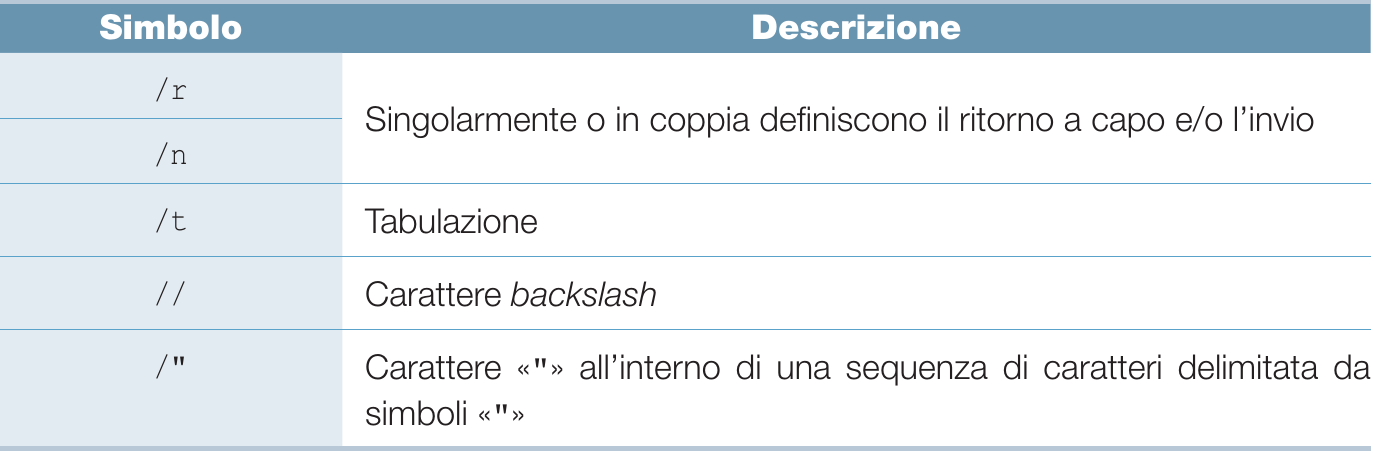
\includegraphics[scale=0.3]{img/escape_sequences.png}
        \end{center}
        \onslide<3->
        È conveniente per il programmatore scrivere il ritorno a capo con \mintinline{cpp}{endl}.
    \end{frame}

    \begin{frame}[fragile]
        \frametitle{Input}
        L'input in un programma è svolto tramite il comando \mintinline{cpp}{cin} e la sintassi è:
        \onslide<2->
        \begin{cppcode}
            int i = 0;
            cout << "Inserire il numero di patate comprate: ";
            cin >> i;
        \end{cppcode}
        \onslide<3->
        \begin{block}{Attenzione}
            Non è possibile concatenare una richiesta input come si fa con l'output.
        \end{block}
    \end{frame}

    \begin{frame}
        \frametitle{Concetti del flusso di esecuzione}
        Al momento noi abbiamo già visto diversi modi di eseguire il nostro codice, il primo tra tutti è quello in \textbf{sequenza}. Di fatto noi inseriamo i comandi fino a quando questi non finiscono.
    \end{frame}

    \begin{frame}[fragile]
        \frametitle{La selezione}
        La selezione è l'esecuzione del codice quando viene soddisfatta una determinata condizione. In poche parole, utilizzato gli \mintinline{cpp}{if}, siamo in grado di condizionare l'esecuzione del nostro codice.
        \onslide<2->
        \begin{cppcode}
            // Piccolo programma che se feature è 0, sappiamo che qualcosa è disattivato
            const int feature = 0;
            if (feature == 0) {
                cout << "Funzionalità disattivata";
            }
        \end{cppcode}
    \end{frame}

    \begin{frame}[fragile]
        \frametitle{La selezione, \mintinline{cpp}{else} e \mintinline{cpp}{else if}}
        Possiamo anche definire cosa succede nel caso il nostro \mintinline{cpp}{if} non sia soddisfatto tramite l'\mintinline{cpp}{else}:
        \onslide<2->
        \begin{cppcode}
            const int feature = 0;
            if (feature == 0) {
                cout << "Funzionalità disattivata";
            } else {
                cout << "Funzionalità attiva";
            }
        \end{cppcode}
    \end{frame}

    \begin{frame}[fragile]
        \frametitle{La selezione, \mintinline{cpp}{else} e \mintinline{cpp}{else if}}
        Possiamo pure mettere in combinazione \mintinline{cpp}{if} e \mintinline{cpp}{else} per le casistiche più particolari:
        \onslide<2->
        \begin{cppcode}
            const int feature = 0;
            if (feature == 0) {
                cout << "Funzionalità disattivata";
            } else if (feature == 1) {
                cout << "Funzionalità attiva";
            } else {
                cout << "Codice funzionalità errato";
            }
        \end{cppcode}
    \end{frame}

    \begin{frame}
        \frametitle{Casistiche multiple}
        Ci sono casi dove dobbiamo passare le nostre variabili attraverso una lunga lista di \mintinline{cpp}{if}, possiamo rendere il nostro codice più leggibile con lo \mintinline{cpp}{switch}. 
    \end{frame}

    \begin{frame}[fragile]
        \frametitle{Casistiche multiple}
        \begin{cppcode}
            char selezione;
            cin >> selezione;
            switch (selezione)
            {
                case 'A':
                    cout << "Eseguo A...";
                    break;
                case 'B':
                    cout << "Eseguo B...";
                    break;
                default:
                    cout << "Selezione invalida!";
                    break;
            }
        \end{cppcode}
    \end{frame}

    \begin{frame}[fragile]
        \frametitle{Operatore ternario}
        Va citato per referenza anche l'operatore ternario, il quale ci aiuta a rendere più snello il nostro codice. È uno strumento principalmente usato per assegnare delle variabili in maniera condizionale. Senza definire in maniera rigida la sintassi, un esempio è molto più semplice.
    \end{frame}

    \begin{frame}[fragile]
        \frametitle{Esempio di operatore ternario}
        \begin{cppcode}
            int i = 0;
            if(<condizione>) {
                i = <valore>;
            } else {
                i = <altroValore>;
            }
        \end{cppcode}
        \onslide<2->
        \begin{cppcode}
            int i = <condizione> ? <valore> : <altroValore>;
        \end{cppcode}
    \end{frame}

    \begin{frame}[fragile]
        \frametitle{Le ripetizioni}
        Sul fronte delle ripetizioni, ci sono tre strutture che ci permettono effettuare cicli del nostro programma.
        \begin{itemize}
            \item<2-> \mintinline{cpp}{while}
            \item<3-> \mintinline{cpp}{do while}
            \item<4-> \mintinline{cpp}{for}
        \end{itemize}
    \end{frame}

    \begin{frame}[fragile]
        \frametitle{\mintinline{cpp}{while}}
        Il \mintinline{cpp}{while} è la struttura ripetitiva più semplice. Basta inserire all'interno una condizione, il ciclo si ripeterà fino a quando la condizione rimane vera durante l'esecuzione. Per entrare dentro il ciclo, la condizione deve essere \textbf{inizialmente vera}.
        \onslide<2->
        \begin{cppcode}
            while (<condizione>) {
                // Codice da ripetere
            }
        \end{cppcode}
        \begin{alertblock}<3->{Attenzione}
            Se la condizione rimane sempre uguale all'interno del \mintinline{cpp}{while}, \textbf{il ciclo eseguirà all'infinito}.
        \end{alertblock}
    \end{frame}

    \begin{frame}[fragile]
        \frametitle{\mintinline{cpp}{do while}}
        Il \mintinline{cpp}{do while} è una struttura che permette di eseguire il primo ciclo del while a prescindere dalla condizione.
        \onslide<2->
        \begin{cppcode}
            do {
                // Codice da ripetere
            } while (<condizione>);
        \end{cppcode}
        \begin{block}<3->{Info}
            Solitamente questo tipo di ciclo si utilizza quando si deve eseguire l'operatione all'interno del ciclo almeno una volta. 
        \end{block}
    \end{frame}

    \begin{frame}[fragile]
        \frametitle{\mintinline{cpp}{for}}
        Il ciclo \mintinline{cpp}{for} è il ciclo più usato solitamente, riprende la logica del \mintinline{cpp}{while} ma impone all'utente di definire la variabile che viene utilizzata per il ciclo e l'incremento per ogni iterazione.
        \onslide<2->
        \begin{cppcode}
            for (int i = 0; i < <valore>; i++) {
                // Codice da ripetere
            }
        \end{cppcode}
    \end{frame}

    \begin{frame}[fragile]
        \frametitle{Interruzione o continuazione di un ciclo}
        Esistono due keyword che permettono di modificare il comportamento di un ciclo: \mintinline{cpp}{break} e \mintinline{cpp}{continue}.
    \end{frame}

    \begin{frame}[fragile]
        \frametitle{\mintinline{cpp}{break} all'interno di un ciclo}
        La keyword \mintinline{cpp}{break} è utilizzata per interrompere il nostro ciclo e uscire dallo stesso.
        \onslide<2->
        \begin{cppcode}
            while (true) {
                char character;
                cin >> character;
                if (character == 'q') {
                    break;
                }
            }
        \end{cppcode}
    \end{frame}

    \begin{frame}[fragile]
        \frametitle{\mintinline{cpp}{continue}}
        Continue invece, è utilizzata per passare alla prossima iterazione del nostro ciclo.
        \onslide<2->
        \begin{cppcode}
            for (int i = 0; i <= 100; i++) {
                if (i % 2 == 1) {
                    continue;
                }
                cout << i << endl;
            }
        \end{cppcode}
    \end{frame}

\end{document}